
\documentclass[a4paper, fleqn]{article}

% Поля
\usepackage[left=1.5cm, right=1.5cm, top=1.5cm, bottom=1.5cm, bindingoffset=1cm]{geometry}

\usepackage[utf8]{inputenc} % UTF-8
\usepackage[T1, T2A]{fontenc}   % UTF-8
\RequirePackage[english,russian]{babel}

%\usepackage{amsfonts}
%\usepackage{bm}              % Верхнее подчёркивание
\usepackage{setspace}         % Отступы
\usepackage{amssymb,graphicx} % Точки, ромбики...
\usepackage{amsmath}          % Система уравнений
\usepackage{mathtools}        % Переносы в формулах
\usepackage{amsmath}          % Переносы в формулах
\usepackage{listings}         % Подсветка кода
\RequirePackage{verbatim}
\usepackage{color}
\usepackage{graphicx}
\usepackage{amsmath, amsfonts, amssymb}
\usepackage{mathtext}
\usepackage{tocloft}
\usepackage{hyperref}
\usepackage{indentfirst}
\usepackage{caption}
\usepackage{multirow}
\usepackage{here}
\usepackage{array}
\usepackage{lscape}

\usepackage[dvipsnames]{xcolor}

% Шрифты без засечек и ровные формулы
\usepackage{concmath, concrete}
\usepackage{euler}

% dots in tableofcontents
\renewcommand{\cftsecleader}{\cftdotfill{\cftdotsep}}

% Надоть
\RequirePackage{textcomp}

\setcounter{tocdepth}{3}

% Межстрочный интервал
\setlength{\abovedisplayskip}{3pt}
\setlength{\belowdisplayskip}{3pt}
\setlength\abovedisplayshortskip{3pt}
\setlength\belowdisplayshortskip{3pt}


\lstset{
  literate={а}{{\selectfont\char224}}1
           {б}{{\selectfont\char225}}1
           {в}{{\selectfont\char226}}1
           {г}{{\selectfont\char227}}1
           {д}{{\selectfont\char228}}1
           {е}{{\selectfont\char229}}1
           {ё}{{\"e}}1
           {ж}{{\selectfont\char230}}1
           {з}{{\selectfont\char231}}1
           {и}{{\selectfont\char232}}1
           {й}{{\selectfont\char233}}1
           {к}{{\selectfont\char234}}1
           {л}{{\selectfont\char235}}1
           {м}{{\selectfont\char236}}1
           {н}{{\selectfont\char237}}1
           {о}{{\selectfont\char238}}1
           {п}{{\selectfont\char239}}1
           {р}{{\selectfont\char240}}1
           {с}{{\selectfont\char241}}1
           {т}{{\selectfont\char242}}1
           {у}{{\selectfont\char243}}1
           {ф}{{\selectfont\char244}}1
           {х}{{\selectfont\char245}}1
           {ц}{{\selectfont\char246}}1
           {ч}{{\selectfont\char247}}1
           {ш}{{\selectfont\char248}}1
           {щ}{{\selectfont\char249}}1
           {ъ}{{\selectfont\char250}}1
           {ы}{{\selectfont\char251}}1
           {ь}{{\selectfont\char252}}1
           {э}{{\selectfont\char253}}1
           {ю}{{\selectfont\char254}}1
           {я}{{\selectfont\char255}}1
           {А}{{\selectfont\char192}}1
           {Б}{{\selectfont\char193}}1
           {В}{{\selectfont\char194}}1
           {Г}{{\selectfont\char195}}1
           {Д}{{\selectfont\char196}}1
           {Е}{{\selectfont\char197}}1
           {Ё}{{\"E}}1
           {Ж}{{\selectfont\char198}}1
           {З}{{\selectfont\char199}}1
           {И}{{\selectfont\char200}}1
           {Й}{{\selectfont\char201}}1
           {К}{{\selectfont\char202}}1
           {Л}{{\selectfont\char203}}1
           {М}{{\selectfont\char204}}1
           {Н}{{\selectfont\char205}}1
           {О}{{\selectfont\char206}}1
           {П}{{\selectfont\char207}}1
           {Р}{{\selectfont\char208}}1
           {С}{{\selectfont\char209}}1
           {Т}{{\selectfont\char210}}1
           {У}{{\selectfont\char211}}1
           {Ф}{{\selectfont\char212}}1
           {Х}{{\selectfont\char213}}1
           {Ц}{{\selectfont\char214}}1
           {Ч}{{\selectfont\char215}}1
           {Ш}{{\selectfont\char216}}1
           {Щ}{{\selectfont\char217}}1
           {Ъ}{{\selectfont\char218}}1
           {Ы}{{\selectfont\char219}}1
           {Ь}{{\selectfont\char220}}1
           {Э}{{\selectfont\char221}}1
           {Ю}{{\selectfont\char222}}1
           {Я}{{\selectfont\char223}}1
}

\definecolor{mygreen}{rgb}{0,0.6,0}
\definecolor{mygray}{rgb}{0.5,0.5,0.5}
\definecolor{mymauve}{rgb}{0.58,0,0.82}

% dots in tableofcontents
\renewcommand{\cftsecleader}{\cftdotfill{\cftdotsep}}

\lstset{ 
  backgroundcolor=\color{white},      % choose the background color; you must add \usepackage{color} or \usepackage{xcolor}; should come as last argument
  basicstyle=\footnotesize\ttfamily,  % the size of the fonts that are used for the code
  breakatwhitespace=false,         % sets if automatic breaks should only happen at whitespace
  breaklines=true,                 % sets automatic line breaking
  captionpos=b,                    % sets the caption-position to bottom
  commentstyle=\color{mygreen},    % comment style
  deletekeywords={...},            % if you want to delete keywords from the given language
  escapeinside={\%*}{*)},          % if you want to add LaTeX within your code
  extendedchars=true,              % lets you use non-ASCII characters; for 8-bits encodings only, does not work with UTF-8
  frame=single,	                   % adds a frame around the code
  keepspaces=true,                 % keeps spaces in text, useful for keeping indentation of code (possibly needs columns=flexible)
  keywordstyle=\color{blue},       % keyword style
  language=Octave,                 % the language of the code
  morekeywords={*,...},            % if you want to add more keywords to the set
  numbers=left,                    % where to put the line-numbers; possible values are (none, left, right)
  numbersep=5pt,                   % how far the line-numbers are from the code
  numberstyle=\tiny\color{mygray}, % the style that is used for the line-numbers
  rulecolor=\color{black},         % if not set, the frame-color may be changed on line-breaks within not-black text (e.g. comments (green here))
  showspaces=false,                % show spaces everywhere adding particular underscores; it overrides 'showstringspaces'
  showstringspaces=false,          % underline spaces within strings only
  showtabs=false,                  % show tabs within strings adding particular underscores
  stepnumber=2,                    % the step between two line-numbers. If it's 1, each line will be numbered
  stringstyle=\color{mymauve},     % string literal style
  tabsize=2,	                   % sets default tabsize to 2 spaces
  %title=\lstname                   % show the filename of files included with \lstinputlisting; also try caption instead of title
}

\makeatletter



\begin{document}
\large

\begin{titlepage}
  \begin{center}
    \large
    Санкт-Петербургский политехнический университет Петра Великого\\
    Кафедра компьютерных систем и программных технологий
    
    \vfill
 
    \textsc{\bf \LARGE Отчёт по курсовой работе}\\[5mm]
     
    {
    
    \Large {\bf Дисциплина:} Низкоуровневое программирование\\[2mm]
    {\bf Тема:} Симулятор 8-битного процессора intel 8051 
    
    }
  \bigskip
     
    %Нестандартный практикум, 2 курс, группа 777
\end{center}
\vfill
 
\newlength{\ML}
\settowidth{\ML}{«\underline{\hspace{0.7cm}}» \underline{\hspace{2cm}}}
\hfill\begin{minipage}{0.4\textwidth}
  Выполнил студент гр. 23531/2\\
  \underline{\hspace{\ML}} Н.С. Макаревич\\
\end{minipage}
\bigskip
 
\hfill\begin{minipage}{0.4\textwidth}
  Преподаватель\\
  \underline{\hspace{\ML}} М.Х. Ахин\\
  «\underline{\hspace{0.7cm}}» \underline{\hspace{2cm}} 2018 г.
\end{minipage}%
\vfill
 
\begin{center}
  Санкт-Петербург, 2018 г.
\end{center}
\end{titlepage}


\setcounter{page}{2}

\tableofcontents
\newpage


\section{Задание}
Реализовать симулятор работы процессора intel 8051. Содержимое памяти задается и выводится в текстовый файл. Формат файла фиксируется в ТЗ. \\
Необходимо обеспечить возможность имитации работы процессора до останова (HLT) или в течение заданного числа шагов (инструкций). Необходимо обеспечить возможность отладки машины (вывод содержимого памяти и регистров, возобновление работы машины). \\
Задание не предполагает имитацию ввода-вывода и контроллера прерываний.

\section{Описание функциональности симулятора}
Данный симулятор процессора intel 8051 способен запускать программы либо из бинарного файла прошивки микроконтроллера (образ памяти программ), либо из специального текстового формата. \\
Пользователь составляет файл, описывающий состояние памяти устройства в начальный момент времени. Бинарный файл прошивки содержит только образ памяти программ и воспринимается симулятором как состояние процессора в начальный момент времени. \\
Текстовый формат содержит информацию о состоянии памяти программ, памяти данных, регистров и счётчика инструкций, так что может быть использован в качестве снимка состояния процессора в определённый момент времени. \\
Симулятор позволяет просматривать последовательность выполняемых инструкций, менять скорость выполнения программы, а также исполнять программу пошагово -- по одной инструкции. \\
Пользователь может остановить программу в нужном месте, нажав клавишу Enter, указав необходимый адрес в текстовом файле, а также при помощи аргументов командной строки. Пока программа остановлена, можно просматривать состояние памяти программ и памяти данных, а также делать снимки состояния. \\
По умолчанию память программ имеет размер 4 Кбайта, а память данных -- 256 байт, но при необходимости их можно расширить до 64 Кбайт. \\
Большинство прошивок микроконтроллера находится в формате intel hex, но их можно легко перевести в бинарный файл (например, с помощью программы objcopy).

\section{Система команд процессора}
Набор инструкций, которые может обрабатывать симулятор, должен соответсововать тому набору инструкций, которыми оперирует реальный процессор intel 8051.\\
Описание всех инструкций, регистров и поведения процессора приведено в книге \\[5mm]
Горюнов А.Г., Ливенцов С.Н. Архитектура микроконтроллера Intel 8051 \\
Томск: Изд-во ТПУ, 2005. - 86 с. \\

\section{Работа с симулятором}
\subsection{Аргументы командной строки}
\begin{enumerate}
	\item[{\tt\bf -h}] {-}-help \\
	Показать краткую справку по командам симулятора. \\
	Выводит в консоль содержимое файла resources/help.txt
	
	\item[{\tt\bf -d}] {-}-debug \\
	Включает отладочные средства (реакцию на брэйкпойнты, вывод в консоль).
	Если флаг не  установлен, то симулятор исполняет программу, ничего не выводя в консоль.
	
	\item[{\tt\bf -i}] {-}-infile \\
	Имя входного файла. \\
	Пример: -i myfile
	
	\item[{\tt\bf -o}] {-}-outfle \\
	Имя выходного файла. \\ 
	Так будет называться файл образа памяти, полученный после завершения программы. Если пользователь делает промежуточные снимки состояния процессора, то в начало имени файла добавляются дата, время и номер дампа.\\
	Имя файла по-умолчанию -- "memory".\\
	Пример: -o myfile
	
	\item[{\tt\bf -c}] {-}-clk \\
	Время задержки между исполнением инструкций. Количество милисекунд, целое беззнаковое число. По умолчанию задержки нет.\\
	Пример: -c 1000
	
	\item[{\tt\bf -v}] {-}-verbose \\
	Verbose режим. Отображает в реальном времени последовательность машинных команд, которые исполняет процессор. По умолчанию выключен.
	
	\item[{\tt\bf -m}] {-}-mode \\
	Тип принимаемого на вход файла (bin или text) \\
	Пример: -m bin
	
	\item[{\tt\bf -b}] {-}-break \\
	Добавление брэйкпойнтов \\
	В этом параметре передаётся адрес в шестнадцатеричном виде. На этом адресе будет добавлен брэйкпойнт. \\
	$^\wedge$ означает, что брэйкпойнт сработает перед исполнением соответствующей инструкции. \_ означает, что он сработает после её исполнения. \\
	Пример: -b $^\wedge2C$
	
	\item[{\tt\bf {-}-nobreak}]
	Игнорирование брэйкпойнтов \\
	С этим флагом программа не будет останавливаться на брэйкпойнтах, обозначенных пользователем в файле или в командной строке.
	
	\item[{\tt\bf -s}] {-}-save \\
	Добавление cэйвпойнтов \\
	В этом параметре передаётся адрес в шестнадцатеричном виде. На этом адресе будет сделан снимок состояния процессора. \\
	$^\wedge$ означает, что снимок будет сделан перед исполнением соответствующей инструкции. \_ означает, что он будет сделан после её исполнения. \\
	Пример: -s {\_}2C
	
	\item[{\tt\bf -z}] {-}-convert \\
	С этим флагом симулятор не исполняет программу, а просто преобразует входной бинарный файл в текстовый файл - образ памяти.\\

	\item[{\tt\bf -e}] {-}-end \\
	Задание конечного адреса программы. \\
	Адрес задаётся как шестнадцатеричное неотрицательное число. \\
	Если счётчик PC превысит это значение, то программа будет остановлена, а конечное состояние сохранено в файл. \\
	Пример: -e E6
	
	\item[{\tt\bf {-}-epm}]
	Флаг, включающий поддержку внешней памяти программ.
	
	\item[{\tt\bf {-}-edm}]
	Флаг, включающий поддержку внешней памяти данных.
	
	\item[{\tt\bf {-}-step}]
	Step-by-step режим. С этим флагом программа будет исполняться по одной инструкции по нажатию клавиши Enter.\\
	Брэйкпойнты генерируются после каждой исполненной инструкции.
	
\end{enumerate}

\subsection{Интерфейс}
Симулятор имеет консольный интерфейс. \\
Если флаги -d и -v не установлены, то в консоль ничего не  выводится. Программа исполняется без временных задержек и конечное состояние процессора записывается в выходной файл. \\
Если установлен флаг -d (debug), то в консоль будет выводиться информация о брэйкпойнтах и сэйвпойнтах. \\
Если же установлены флаги -d и -v (verbose), то в консоль будут выводиться инструкции, которые исполняет процессор. \\
\newpage
Пример вывода программы:
\begin{figure}[H]
	\centering
	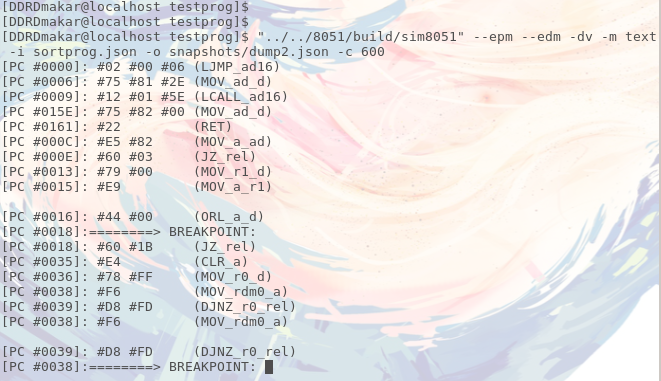
\includegraphics[width=0.8\linewidth]{img/interface}
	\caption{}
\end{figure}
В квадратных скобках выведено значение счётчика инструкций PC. Затем в строке представлены коды инструкций, они могут состоять из одного, двух или трёх байт. Последней в строке указывается мнемоника в круглых скобках, соответствующая данной инструкции (Для случая, когда программа запущена из текстового файла). \\
Если пользователю требуется остановить исполнение инструкций, достаточно нажать клавишу Enter -- это вызовет Breakpoint в текущем месте программы. \\
Когда программа остановлена на брэйкпойнте, то пользователь может использовать команды для просмотра памяти и сохранения состояния. Они описаны ниже в разделе о брэйкпойнтах.


\section{Текстовый формат снимка состояния симулятора}
Снимок состояния микроконтроллера intel 8051 \\ представляет собой JSON-структуру вида:\\
\begin{lstlisting}
{
	"PC": "#.."
	"rga": "#..",
	"rgb": "#..",
	"rgc": "#..",
	...
	
	"program": "...",
	"data": "..."
}
\end{lstlisting}

Состояние счётчика инструкций (PC), памяти программы (program) и памяти данных (data) задаётся в специальном текстовом формате. \\
Значения регистров указываются в виде шестнадцатеричного числа в строке. \\
Память программы и память данных заданы в виде строк, содержащих мнемокоды инструкций и числовые константы. Пробелы, табуляция и переносы строки используются в качестве разделителя.

\subsection{Числа и инструкции в памяти}
Обычное число (8 двоичных разрядов) может быть записано в виде:
~
~\\[3mm]
\begin{tabular}{{l}{l}}
	Шестнадцатеричного числа: & {\tt\large \#FF} \\[2mm]
	Двоичного числа:          & {\tt\large 11111111} \\[2mm]
	Десятичного числа:        & {\tt\large *255} \\
\end{tabular} \\[3mm]
~
Числа должны быть целыми и неотрицательными. Если симулятор прочтёт число больше 255, то программа завершится с ошибкой.\\
~\\
Также пользователь может писать названия инструкций и регистров. Инструкции разделяются пробелами, символами табуляции или переносом строки. Регистр букв не учитывается.\\
Соответствие мнемоник инструкциям задаётся в специальном конфигурационном файле resources/mnemonics.json \\
Значения регистров представлены в файле отдельно для удобства, но при этом продублированы в памяти данных. \\
Если значение регистра указано отдельно, то оно обладает более высоким приоритетом, чем значения в памяти данных.

\subsection{Определение мнемокодов}
Мнемокоды, соответствующие определённым инструкциям, задаются пользователем в конфигурационном файле resources/mnemonics.json. \\
Пользователь может на своё усмотрение назначить соответствие различных символьных строк кодам от 0 до 255. \\
Когда симулятор стартует из текстового файла, то по очереди парсит инструкции, заданные в текстовом формате. Если код инструкции или константы указан в виде числа, например 1101 или \#FF, то он сразу декодируется и попадает в память. Если же программа встречает строку, то ищет соответствующий ей код в файле mnemonics.json. \\
Все мнемокоды должны быть указаны в нижнем регистре.
\paragraph{Формат файла mnemonics.json}~\\
\begin{lstlisting}
{
	"nop": 0,	
	"ajmp_ad11_0": 1,
	"ljmp_ad16":   2,
	"rr_a":   3,
	"inc_a":  4,
	"inc_ad": 5,
	"acc":    224
}
\end{lstlisting}
Здесь мы указываем мнемокод как ключ и соответствующий ему код как значение (целое неотрицательное число). 

\newpage
\subsection{Брэйкпойнты}
В текстовое представление можно добавлять точки останова программы (breakpoint). Когда программа доходит до брэйкпойнта, то приостанавливается и пользователь может выполнять некоторые действия, прежде чем запустит ход выполнения программы дальше.\\
Можно просматривать значения, хранящиеся в определённых ячейках памяти программ и памяти данных. Для этого необходимо написать букву <<p>> или <<d>>, которые указывают на место, откуда мы читаем значение. <<p>> - из памяти программы, <<d>> - из памяти данных. \\
Далее после буквы пользователь должен указать адрес ячейки в шестнадцатеричном виде и нажать клавишу Enter. \\
Например, чтобы прочитать из памяти данных значение, находящееся по адресу 88, достаточно написать d88 . \\
Также после остановки программы на брэйкпойнте пользователь может сохранить состояние процессора в файл, написав команду "save". \\
Команда "step" позволяет включать/выключать режим пошагового исполнения инструкций. \\
Брэйкпойнт в текстовом файле записывается в формате $^\wedge$BREAK или \_BREAK \\
Символ $^\wedge$ ставится перед BREAK, если программа должна быть приостановлена после предыдущей инструкции, а символ \_ ставится, если программа должна быть приостановлена перед следующей инструкцией.

\subsection{Точки сохранения снимка памяти}
Можно добавлять в код точки сохранения (savepoint). Когда программа доходит до сейвпойнта, то дампит в текстовый файл состояние памяти и регистров в данный момент.\\
Сейвпойнт записывается в формате $^\wedge$SAVE или \_SAVE \\
Символы $^\wedge$ и \_ выполняют ту же функцию, что и в случае с брэйкпойнтами. \\

{ \it \large
Брэйкпойнты и сейвпойнты не влияют на последовательность инструкций, которую в итоге исполняет процессор. Симулятор держит их в памяти отдельно и отслеживает, когда то или иное правило должно сработать.
}
\\

\subsection{Комментарии}
Пользователь может включать в текст программы комментарии, которые будут проигнорированы симулятором, но сделают код более понятным. Они записываются в одинарных кавычках ('\space'). Комментарий может содержать любые символы кроме одинарных кавычек.
Комментарии будут проигнорированы на этапе перевода текста в бинарный код и никак не повлияют на программу.

\newpage
\paragraph{Пример снимка состояния симулятора}~\\
\lstinputlisting[]{dump.json}

\newpage
\section{Сборка проекта}
Сборка программы, в соответствии с заданием, осуществляется при помощи <<make>>. \\
Для сборки проекта необходимы библиотеки jansson и pthread. \\
Дополнительно требуется указать, под какой тип архитектуры процессора мы компилируем программу, little-endian или big-endian. \\\\
<<make ENDIANNESS=0>> - для little-endian архитектуры. \\
<<make ENDIANNESS=1>> - для big-endian архитектуры. \\
~\\
Опции компилятора:
\begin{lstlisting}
-lm -Os -std=c11 -pedantic -Wextra -Wall -l pthread -l jansson
\end{lstlisting}

\section{Проверка работоспособности симулятора}
Для проверки работоспособности симулятора было написано три программы под микроконтроллер на ядре intel8051 на языке Си. Программу, выполняющую операции над числом в цикле, программу, производящую арифметические операции, и программу сортировки массива пузырьком. \\
Для всех трёх программ известен результат их работы и можно делать выводы, правильный ли результат выдаёт программа, запущенная на симуляторе. \\
Для компиляции программы был использован компилятор sdcc-3.6.0 под архитектуру intel 8051. Затем полученный файл в формате intel hex (.ihx) был переведён в бинарный файл при помощи программы objcopy и запущен на симуляторе. \\
\begin{lstlisting}
objcopy -I ihex file.ihx -O binary file.bin
\end{lstlisting}
~\\
Программы выдают правильный результат. Это значит, что программа работает корректно в данной ситуации и ошибок не происходит. \\
Программы включены в проект и  находятся в папке test.

\newpage

\section{Выводы}
В данной курсовой работе был реализован симулятор работы процессора intel 8051. С его помощью можно запускать программы для микроконтроллеров на ядре 8051 и отлаживать их. Симулятор позволяет отслеживать ход исполнения инструкций в реальном времени, просматривать содержимое памяти и сохранять снимки состояния процессора в файл. \\ Такие возможности недоступны при работе с реальным микроконтроллером. \\
В данном симуляторе не реализована поддержка работы с внешними интерфейсами ввода/вывода и прерываниями, но я планирую продолжать работу над ним. \\

\begin{thebibliography}{}
    \bibitem{} Горюнов А.Г., Ливенцов С.Н. Архитектура микроконтроллера Intel 8051 Томск: Изд-во ТПУ, 2005. - 86 с.
    \bibitem{} http://www.gaw.ru/html.cgi/txt/doc/micros/mcs51/asm/start.htm
\end{thebibliography}

\end{document}
